\documentclass{beamer}

\usepackage{graphicx}
\usepackage{caption}

\begin{document}
	
	\begin{frame}[plain]
		\begin{figure}
			\centering
			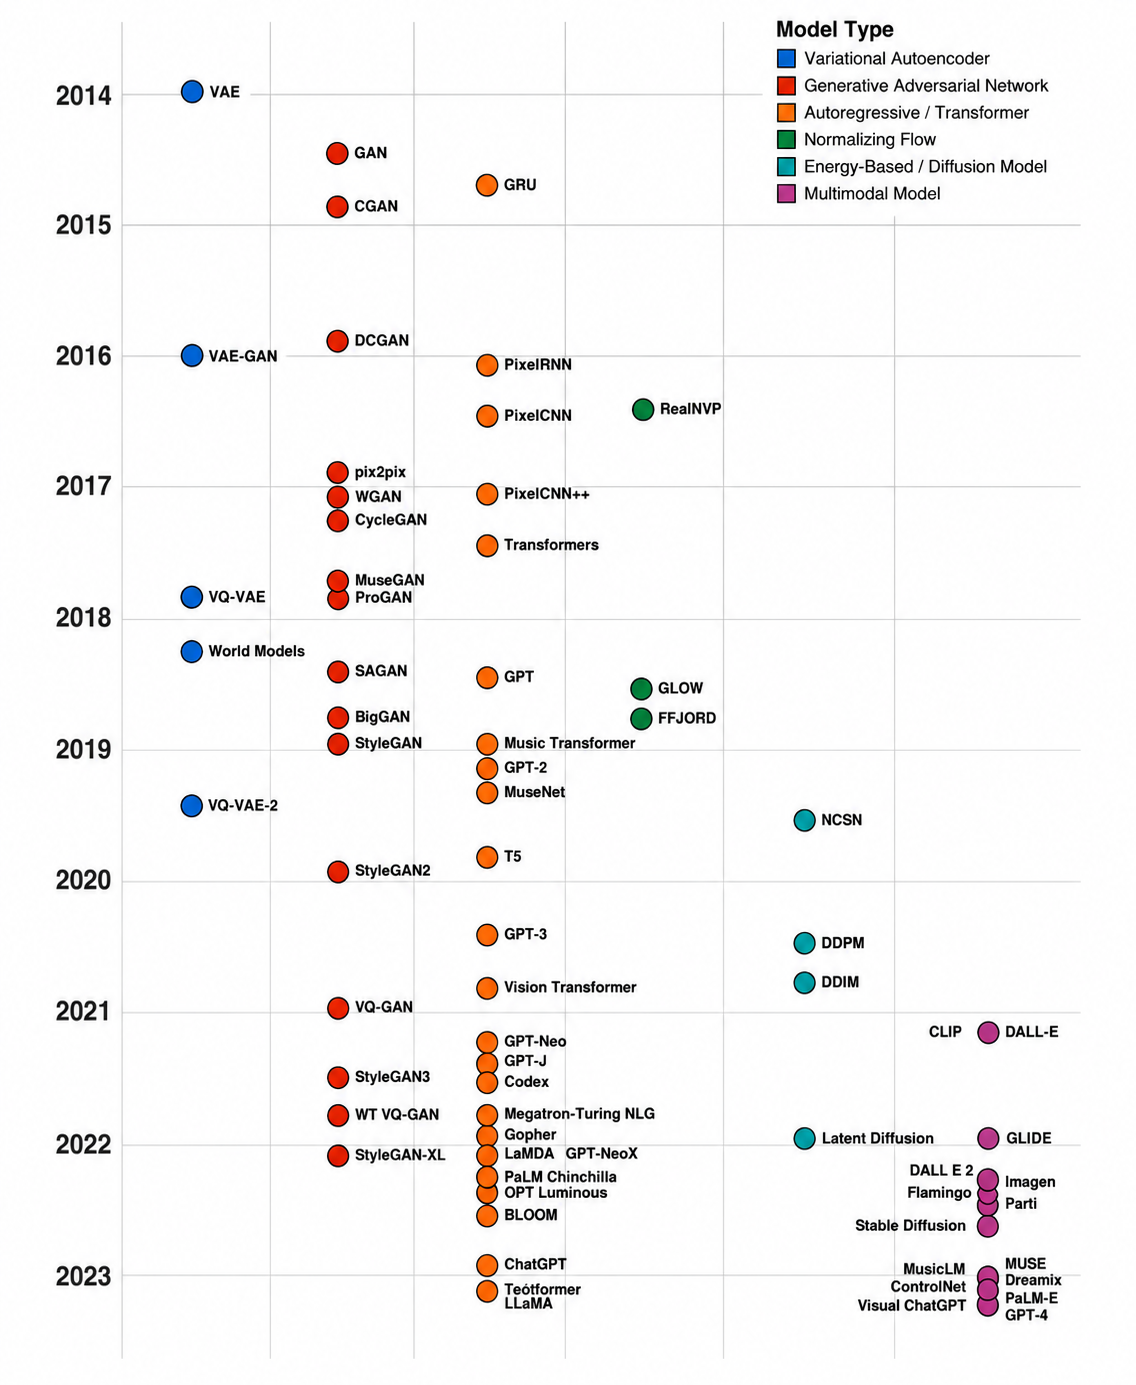
\includegraphics[width=\textwidth,height=0.78\textheight,keepaspectratio]{141.jpg}
			\caption{A brief history of generative AI from 2014 to 2023 (note: some important
				developments such as LSTMs and early energy-based models [e.g., Boltzmann machines]
				precede this timeline)}
		\end{figure}
	\end{frame}
	
	\begin{frame}[plain]
		\begin{figure}
			\centering
			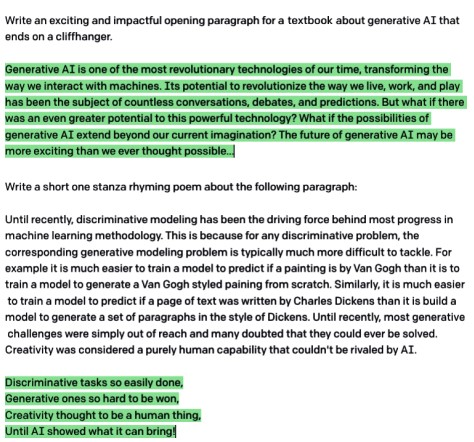
\includegraphics[width=\textwidth,height=0.77\textheight,keepaspectratio]{142.jpg}
			\caption{Output from GPT-3—the non-highlighted text is the prompt and the green
				highlighted text is the output from GPT-3}
		\end{figure}
	\end{frame}
	
	\begin{frame}[plain]
		\begin{figure}
			\centering
			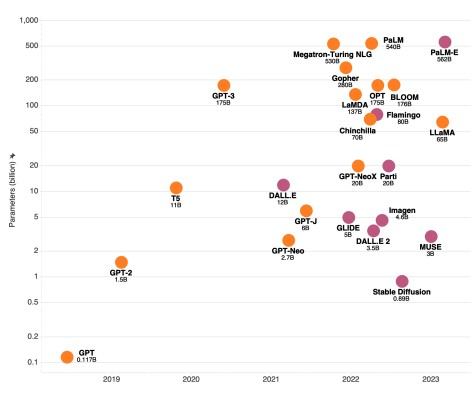
\includegraphics[width=\textwidth,height=0.85\textheight,keepaspectratio]{143.jpg}
			\caption{The size of large language models (orange) and multimodal models (pink)
				in number of parameters over time}
		\end{figure}
	\end{frame}
	
	\begin{frame}[plain]
		\begin{figure}
			\centering
			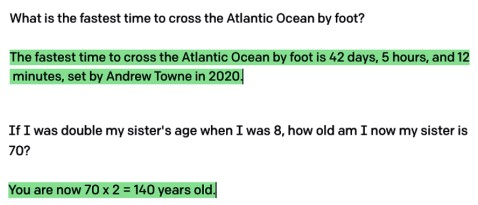
\includegraphics[width=\textwidth,height=0.85\textheight,keepaspectratio]{144.jpg}
			\caption{While large language models excel at some tasks, they are also prone to mis‐
				takes related to factual or logical reasoning (GPT-3 output shown)}
		\end{figure}
	\end{frame}
	
	\begin{frame}[plain]
		\begin{figure}
			\centering
			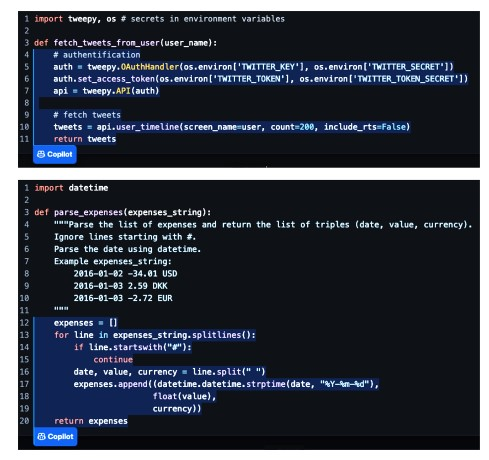
\includegraphics[width=\textwidth,height=0.80\textheight,keepaspectratio]{145.jpg}
			\caption{Two examples of GitHub Copilot capabilities (source: GitHub Copilot)}
		\end{figure}
	\end{frame}
	
	\begin{frame}[plain]
		\begin{figure}
			\centering
			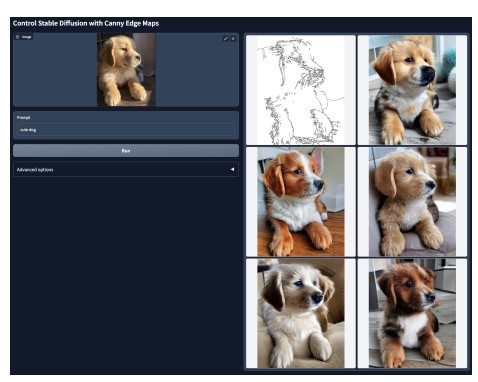
\includegraphics[width=\textwidth,height=0.80\textheight,keepaspectratio]{146.jpg}
			\caption{Conditioning the output of Stable Diffusion using a Canny edge map and
				ControlNet}
		\end{figure}
	\end{frame}
	
	\begin{frame}[plain]
		\begin{figure}
			\centering
			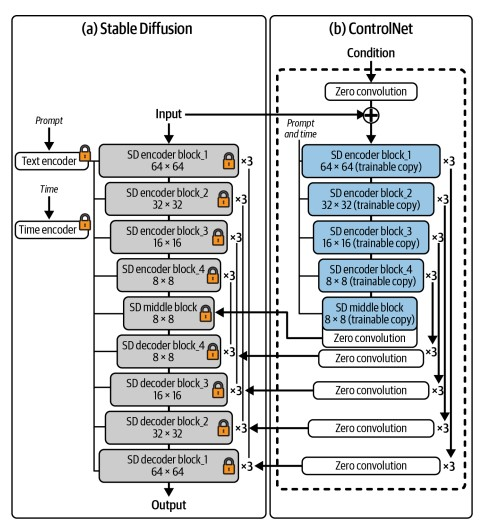
\includegraphics[width=\textwidth,height=0.78\textheight,keepaspectratio]{147.jpg}
			\caption{The ControlNet architecture, with the trainable copies of the Stable Diffusion encoder blocks highlighted in blue}
		\end{figure}
	\end{frame}
	
	\begin{frame}[plain]
		\begin{figure}
			\centering
			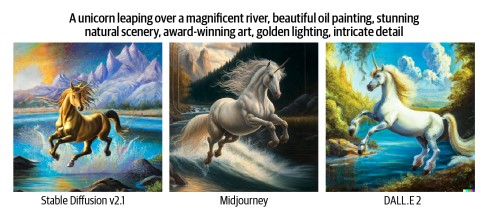
\includegraphics[width=\textwidth,height=0.85\textheight,keepaspectratio]{148.jpg}
			\caption{Outputs from Stable Diffusion v2.1, Midjourney, and DALL.E 2 for the
				same prompt}
		\end{figure}
	\end{frame}
	
	\begin{frame}[plain]
		\begin{figure}
			\centering
			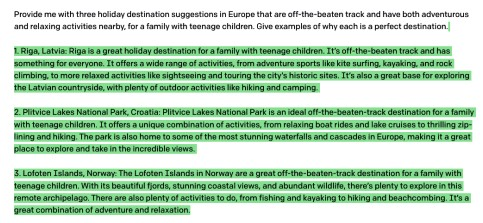
\includegraphics[width=\textwidth,height=0.85\textheight,keepaspectratio]{149.jpg}
			\caption{Output from GPT-3, giving bespoke holiday recommendations}
		\end{figure}
	\end{frame}
	
	\begin{frame}[plain]
		\begin{figure}
			\centering
			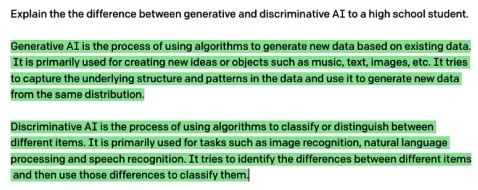
\includegraphics[width=\textwidth,height=0.85\textheight,keepaspectratio]{1410.jpg}
			\caption{Output from GPT-3—an example of how large language models can be
				used for learning}
		\end{figure}
	\end{frame}
	
	\begin{frame}[plain]
		\begin{figure}
			\centering
			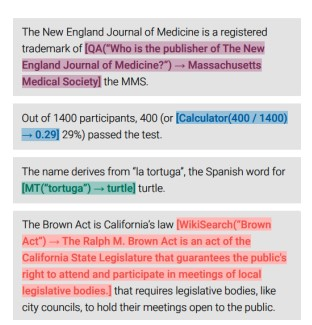
\includegraphics[width=\textwidth,height=0.78\textheight,keepaspectratio]{1411.jpg}
			\caption{An example of how Toolformer is able to autonomously call different APIs
				in order to obtain precise information where necessary}
		\end{figure}
	\end{frame}
	
\end{document}